\chapter{Las moléculas orgánicas: esqueletos y nombres}\label{ch:g11:organic-skeletons}

Un mechero desechable contiene butano, líquido a presión; el cartucho de
un hornillo de camping que se sube a una montaña nevada contiene
propano, o una \omterm{def:g6:pure-substances-and-mixtures:mixture}{mezcla} más rica en él. Los dos están hechos solo de
\omterm{def:g7:atoms-and-molecules:atom}{átomos} de carbono y de hidrógeno, y los dos pertenecen a una enorme
familia: la de las \omterm{def:g7:atoms-and-molecules:molecule}{moléculas} construidas sobre un esqueleto de \omterm{def:g7:atoms-and-molecules:atom}{átomos} de
carbono. Se conocen millones de ellas. Para hablar de ellas, los
químicos necesitan formas de dibujarlas deprisa y de nombrarlas sin
ambigüedad.

\begin{recall}
El carbono forma cuatro \omterm{def:g10:lewis-and-shape:covalent-bond}{enlaces covalentes}, y el hidrógeno, uno;
alrededor de un \omterm{def:g7:atoms-and-molecules:atom}{átomo} de carbono con cuatro enlaces sencillos, los
enlaces apuntan a los vértices de un tetraedro, a unos \ang{109.5}
(\cref{ch:g10:lewis-and-shape}).
\end{recall}

\begin{omfigure}
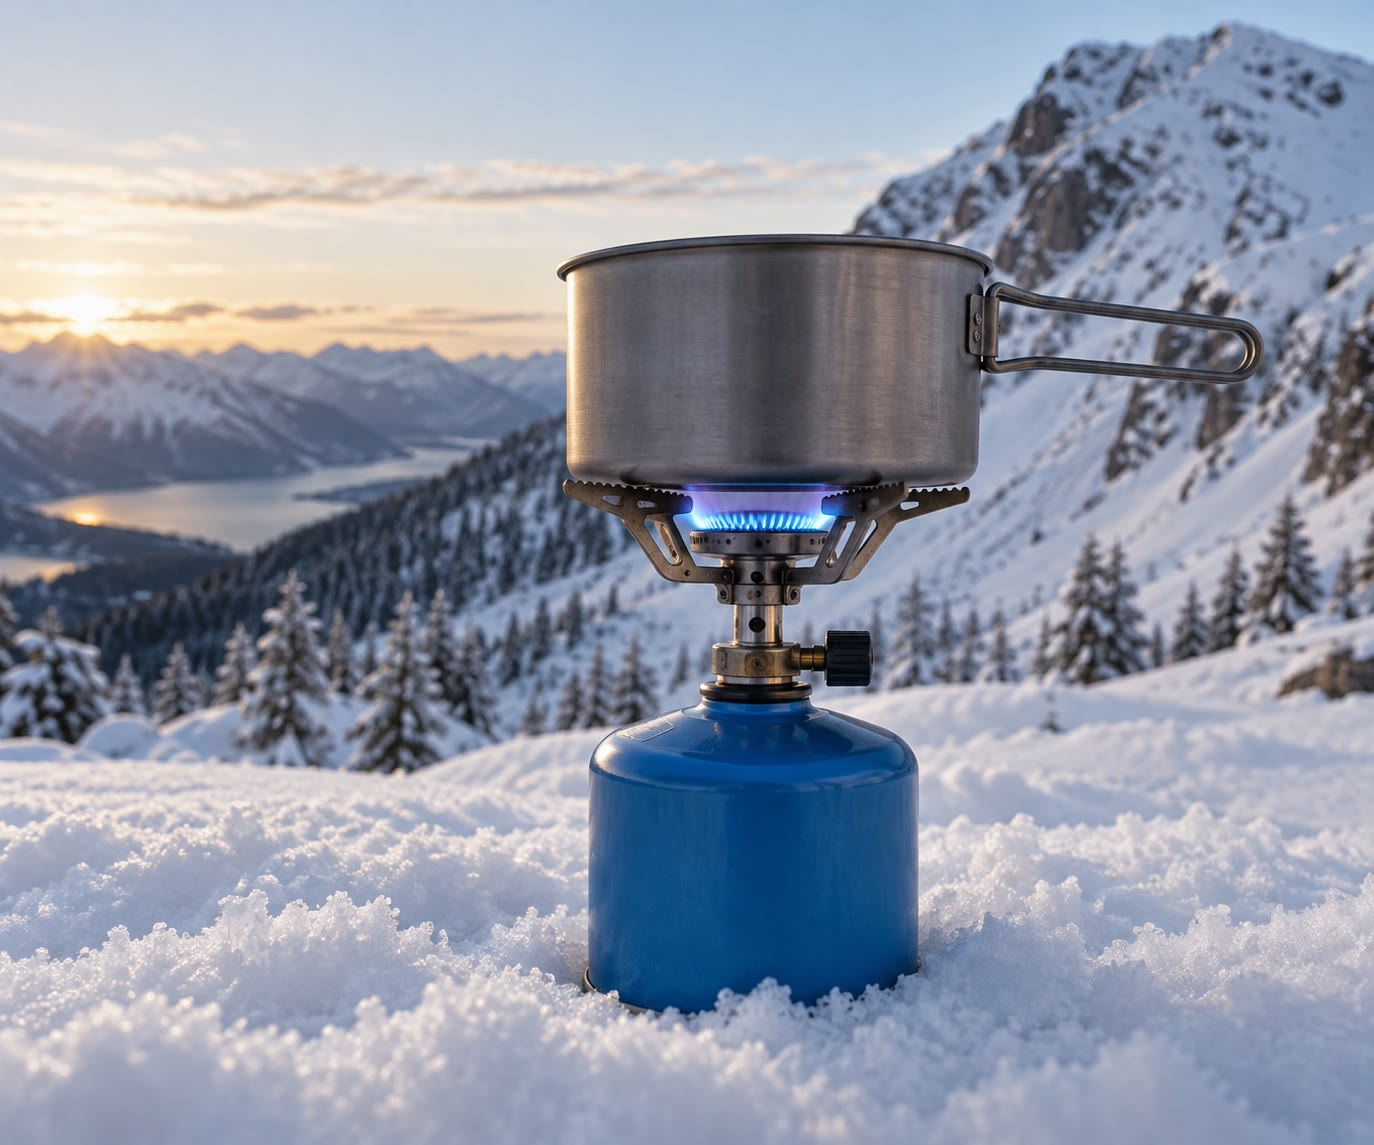
\includegraphics[width=0.48\linewidth]{images/book1/ai/g11-camping-cartridge.jpg}

{\small Un hornillo de camping en la nieve, que quema un gas formado por
carbono e hidrógeno.}
\end{omfigure}

\section{Las fórmulas de las moléculas orgánicas}

\begin{definition}[Compuesto orgánico]\label{def:g11:organic-skeletons:organic}
Un \emph{compuesto orgánico}\index{compuesto organico@compuesto orgánico} es un compuesto
cuyas \omterm{def:g7:atoms-and-molecules:molecule}{moléculas} están construidas sobre un esqueleto de \omterm{def:g7:atoms-and-molecules:atom}{átomos} de
carbono unidos entre sí y a \omterm{def:g7:atoms-and-molecules:atom}{átomos} de hidrógeno, con otros \omterm{def:g7:atoms-and-molecules:atom}{átomos}
posibles como el oxígeno y el nitrógeno. (El dióxido de carbono, el
monóxido de carbono y los carbonatos se dejan fuera por tradición.)
\end{definition}

\begin{definition}[Cuatro tipos de fórmula]\label{def:g11:organic-skeletons:formulas}
Una \omterm{def:g7:atoms-and-molecules:molecule}{molécula} se puede escribir de cuatro maneras:
\begin{itemize}
  \item su \emph{fórmula molecular}\index{formula molecular@fórmula molecular} solo da el
        número de \omterm{def:g7:atoms-and-molecules:atom}{átomos} de cada elemento, como \ce{C4H10};
  \item su \emph{fórmula estructural}\index{formula estructural@fórmula estructural} muestra
        todos los \omterm{def:g7:atoms-and-molecules:atom}{átomos} y todos los enlaces;
  \item su \emph{fórmula semidesarrollada}\index{formula semidesarrollada@fórmula semidesarrollada}
        muestra los enlaces entre \omterm{def:g7:atoms-and-molecules:atom}{átomos} de carbono y agrupa los \omterm{def:g7:atoms-and-molecules:atom}{átomos}
        de hidrógeno con su carbono, como \ce{CH3-CH2-CH2-CH3};
  \item su \emph{fórmula esquelética}\index{formula esqueletica@fórmula esquelética} solo
        dibuja los enlaces del esqueleto carbonado en zigzag: cada
        extremo y cada vértice es un \omterm{def:g7:atoms-and-molecules:atom}{átomo} de carbono, los \omterm{def:g7:atoms-and-molecules:atom}{átomos} de
        hidrógeno unidos al carbono no se dibujan, y todos los demás
        \omterm{def:g7:atoms-and-molecules:atom}{átomos} (con sus \omterm{def:g7:atoms-and-molecules:atom}{átomos} de hidrógeno) se escriben.
\end{itemize}
\end{definition}

\begin{omfigure}
\setchemfig{atom sep=1.45em}
\renewcommand{\arraystretch}{1.6}
\small
\begin{tabular}{@{}l@{\quad}c@{\quad}c@{}}
 & butano & 2-metilpropano \\
molecular & \ce{C4H10} & \ce{C4H10} \\[4pt]
estructural &
\chemfig{H-C(-[2]H)(-[6]H)-C(-[2]H)(-[6]H)-C(-[2]H)(-[6]H)-C(-[2]H)(-[6]H)-H} &
\chemfig{H-C(-[2]H)(-[6]H)-C(-[6]H)(-[2,1.5]C(-[1]H)(-[3]H)(-[2]H))-C(-[2]H)(-[6]H)-H} \\[10pt]
semidesarrollada & \ce{CH3-CH2-CH2-CH3} &
\chemfig{CH_3-CH(-[6]CH_3)-CH_3} \\[14pt]
esquelética & \chemfig{-[:30]-[:-30]-[:30]} & \chemfig{-[:30](-[:90])-[:-30]} \\
\end{tabular}

{\small Las cuatro fórmulas del butano y del 2-metilpropano. En las
\omterm{def:g11:organic-skeletons:formulas}{fórmulas esqueléticas}, cada extremo y cada vértice de los trazos es un
\omterm{def:g7:atoms-and-molecules:atom}{átomo} de carbono: cuatro en cada una.}
\end{omfigure}


\begin{example}[Leer una fórmula esquelética]\label{ex:g11:organic-skeletons:reading}
En la \omterm{def:g11:organic-skeletons:formulas}{fórmula esquelética} del butano, el zigzag tiene dos extremos y dos
vértices: cuatro \omterm{def:g7:atoms-and-molecules:atom}{átomos} de carbono. Cada carbono de un extremo tiene un
enlace dibujado, así que lleva tres \omterm{def:g7:atoms-and-molecules:atom}{átomos} de hidrógeno (\ce{CH3}); cada
vértice tiene dos enlaces dibujados, así que lleva dos (\ce{CH2}). Cada
carbono tiene cuatro enlaces en total, lo que devuelve \ce{C4H10}.
\end{example}

\section{Las cadenas carbonadas}

El esqueleto carbonado de una \omterm{def:g7:atoms-and-molecules:molecule}{molécula} puede ser una cadena
\emph{lineal}, en la que cada carbono está unido como mucho a otros dos,
como en el butano; una cadena \emph{ramificada}, con al menos un carbono
unido a otros tres o cuatro, como en el 2-metilpropano; o un
\emph{anillo}, como en el ciclohexano, \ce{C6H12}, cuya \omterm{def:g11:organic-skeletons:formulas}{fórmula
esquelética} es un hexágono. Para las cadenas se usa un zigzag porque los
enlaces reales alrededor de cada carbono forman ángulos de unos
\ang{109.5}, no de \ang{180}: una cadena ``lineal'' es en realidad un
zigzag en el espacio.

\begin{omfigure}
\setchemfig{atom sep=1.9em}
\begin{tabular}{ccc}
\chemfig{-[:30]-[:-30]-[:30]-[:-30]-[:30]} &
\chemfig{-[:30](-[:90])-[:-30]-[:30](-[:90])-[:-30]} &
\chemfig{*6(------)} \\[4pt]
\small lineal: hexano & \small ramificada: 2,4-dimetilpentano &
\small anillo: ciclohexano \\
\small \ce{C6H14} & \small \ce{C7H16} & \small \ce{C6H12}
\end{tabular}

{\small Tres esqueletos carbonados, en \omterm{def:g11:organic-skeletons:formulas}{fórmulas esqueléticas}.}
\end{omfigure}

\section{Los alcanos y sus nombres}

\begin{definition}[Alcano, grupo alquilo]\label{def:g11:organic-skeletons:alkane}
Un \emph{alcano}\index{alcano} es un compuesto de carbono e hidrógeno
cuyo esqueleto es una cadena (lineal o ramificada, no un anillo) con
solo enlaces sencillos; su \omterm{def:g11:organic-skeletons:formulas}{fórmula molecular} es \ce{C_{n}H_{2n+2}}. Un
\emph{grupo alquilo}\index{grupo alquilo} es lo que queda de un alcano
cuando se le quita un \omterm{def:g7:atoms-and-molecules:atom}{átomo} de hidrógeno, para que pueda unirse a una
cadena: metilo \ce{-CH3}, etilo \ce{-CH2-CH3}.
\end{definition}

\begin{omfigure}
\begin{tabular}{rlcrlc}
\hline
$n$ & nombre & fórmula & $n$ & nombre & fórmula \\
\hline
1 & metano & \ce{CH4}    & 6  & hexano & \ce{C6H14} \\
2 & etano  & \ce{C2H6}   & 7  & heptano & \ce{C7H16} \\
3 & propano & \ce{C3H8}   & 8  & octano & \ce{C8H18} \\
4 & butano  & \ce{C4H10}  & 9  & nonano & \ce{C9H20} \\
5 & pentano & \ce{C5H12}  & 10 & decano & \ce{C10H22} \\
\hline
\end{tabular}\par\medskip

{\small Los diez primeros \omterm{def:g11:organic-skeletons:alkane}{alcanos} lineales. El nombre de una cadena de
$n$ \omterm{def:g7:atoms-and-molecules:atom}{átomos} de carbono es la misma raíz seguida de \emph{-ano}; el \omterm{def:g11:organic-skeletons:alkane}{grupo
alquilo} sustituye \emph{-ano} por \emph{-ilo} (metilo, etilo,
propilo\dots).}
\end{omfigure}

\begin{method}[Nombrar un alcano]\label{met:g11:organic-skeletons:naming}
\begin{enumerate}
  \item Buscar la cadena más larga de \omterm{def:g7:atoms-and-molecules:atom}{átomos} de carbono: da el nombre
        raíz (pentano, hexano\dots).
  \item Los \omterm{def:g7:atoms-and-molecules:atom}{átomos} que no están en ella forman \omterm{def:g11:organic-skeletons:alkane}{grupos alquilo} unidos a
        ella, los sustituyentes.
  \item Numerar la cadena principal desde el extremo que da a los
        sustituyentes los números más bajos.
  \item Escribir cada sustituyente con su número (su posición en la
        cadena), por orden alfabético, delante de la raíz; los grupos
        repetidos llevan los prefijos di-, tri-, tetra-, con un número
        cada uno. Los números se separan con comas, y los números de las
        palabras, con guiones.
\end{enumerate}
\end{method}

\begin{omfigure}
\begin{tikzpicture}[font=\small, x=0.9cm, y=0.9cm]
  % main chain of 5, zigzag; methyls on C2 and C3
  \coordinate (a1) at (0,0); \coordinate (a2) at (0.87,0.5);
  \coordinate (a3) at (1.73,0); \coordinate (a4) at (2.6,0.5);
  \coordinate (a5) at (3.46,0);
  \coordinate (m2) at (0.87,1.5); \coordinate (m3) at (1.73,-1);
  \draw[line width=1pt] (a1) -- (a2) -- (a3) -- (a4) -- (a5);
  \draw[line width=1pt] (a2) -- (m2); \draw[line width=1pt] (a3) -- (m3);
  \foreach \k in {1,2,3,4,5}
    \node[omDef, font=\footnotesize\bfseries, fill=white, inner sep=1pt]
      at ($(a\k)+(0,-0.32)$) {\k};
  \draw[omProp, thick] (m2) circle (0.28);
  \draw[omProp, thick] (m3) circle (0.28);
  \node[omProp, anchor=west] at ($(m2)+(0.35,0)$) {metilo en C2};
  \node[omProp, anchor=west] at ($(m3)+(0.35,0)$) {metilo en C3};
  \node[anchor=west, align=left] at (5,0.3) {cadena más larga: 5 carbonos,
    \emph{pentano}\\ numerada desde la izquierda: 2 y 3\\ (desde la derecha: 3
    y 4, más altos)\\ nombre: \textbf{2,3-dimetilpentano}};
\end{tikzpicture}

{\small Nombrar un \omterm{def:g11:organic-skeletons:alkane}{alcano} ramificado: la cadena principal (numerada),
los sustituyentes (rodeados con un círculo), el nombre.}
\end{omfigure}

\begin{method}[De un nombre a una fórmula esquelética]\label{met:g11:organic-skeletons:drawing}
\begin{enumerate}
  \item Dibujar en zigzag la cadena principal que da la raíz, y numerar
        sus carbonos.
  \item Unir cada sustituyente en la posición que indica su número.
  \item Comprobar: contar los carbonos, y que ningún carbono tenga más de
        cuatro enlaces.
\end{enumerate}
\end{method}

\section{Los isómeros}

\begin{definition}[Isómeros, isómeros constitucionales]\label{def:g11:organic-skeletons:isomer}
Los \emph{isómeros}\index{isomeros@isómeros} son compuestos distintos con la
misma \omterm{def:g11:organic-skeletons:formulas}{fórmula molecular}. Los
\emph{isómeros constitucionales}\index{isomeros constitucionales@isómeros constitucionales} son
isómeros cuyos \omterm{def:g7:atoms-and-molecules:atom}{átomos} están unidos en un orden distinto, por ejemplo
con un esqueleto carbonado distinto.
\end{definition}

\begin{proposition}[Los isómeros tienen propiedades distintas]\label{prop:g11:organic-skeletons:properties}
% ledger: bp:C4H10, bp:isobutane, bp:C5H12, bp:isopentane, bp:neopentane
Los \omterm{def:g11:organic-skeletons:isomer}{isómeros constitucionales} son sustancias distintas, con propiedades
distintas. Entre los \omterm{def:g11:organic-skeletons:alkane}{alcanos} \omterm{def:g11:organic-skeletons:isomer}{isómeros} de una fórmula dada, los más
ramificados hierven a menor temperatura: el butano hierve hacia
\qty{0}{\celsius} y el 2-metilpropano a \qty{-11.7}{\celsius}; el
pentano a \qty{36.1}{\celsius}, el 2-metilbutano a \qty{27.8}{\celsius}
y el 2,2-dimetilpropano a \qty{9.5}{\celsius}.
\end{proposition}

\begin{proof}
Los valores son medidos (registro de datos). Las \omterm{def:g7:atoms-and-molecules:molecule}{moléculas} ramificadas
son más compactas, con menos superficie en contacto con sus vecinas: sus
\omterm{def:g11:polarity-and-cohesion:van-der-waals}{interacciones de van der Waals} son más débiles
(\cref{ch:g11:polarity-and-cohesion}).
\end{proof}

\begin{omfigure}
\setchemfig{atom sep=2em}
\begin{tabular}{ccc}
\chemfig{-[:30]-[:-30]-[:30]-[:-30]} &
\chemfig{-[:30](-[:90])-[:-30]-[:30]} &
\chemfig{-[:0](-[:90])(-[:-90])-[:0]} \\[24pt]
\small pentano & \small 2-metilbutano & \small 2,2-dimetilpropano \\
\small \qty{36.1}{\celsius} & \small \qty{27.8}{\celsius} &
\small \qty{9.5}{\celsius}
\end{tabular}
\medskip

{\small Los tres \omterm{def:g11:organic-skeletons:isomer}{isómeros} de \ce{C5H12} y sus temperaturas de
ebullición: cuanto más ramificado, más baja.}
\end{omfigure}

\section{Los alcanos del petróleo}

El petróleo es una \omterm{def:g6:pure-substances-and-mixtures:mixture}{mezcla} de miles de compuestos, la mayoría \omterm{def:g11:organic-skeletons:alkane}{alcanos} de
1 a más de 40 \omterm{def:g7:atoms-and-molecules:atom}{átomos} de carbono. En una refinería se calienta, y sus
vapores suben por una columna alta, cada vez más fría hacia arriba: cada
fracción se condensa a la altura en la que la temperatura corresponde a
su intervalo de ebullición. Los gases (del metano al butano) salen por
arriba; después, la gasolina, el queroseno y el gasóleo; los aceites
pesados y el betún se quedan abajo. Esta \omterm{def:g10:chemical-species:distillation}{destilación} fraccionada separa
por temperatura de ebullición, que en los \omterm{def:g11:organic-skeletons:alkane}{alcanos} crece con la longitud
de la cadena.

\begin{omfigure}
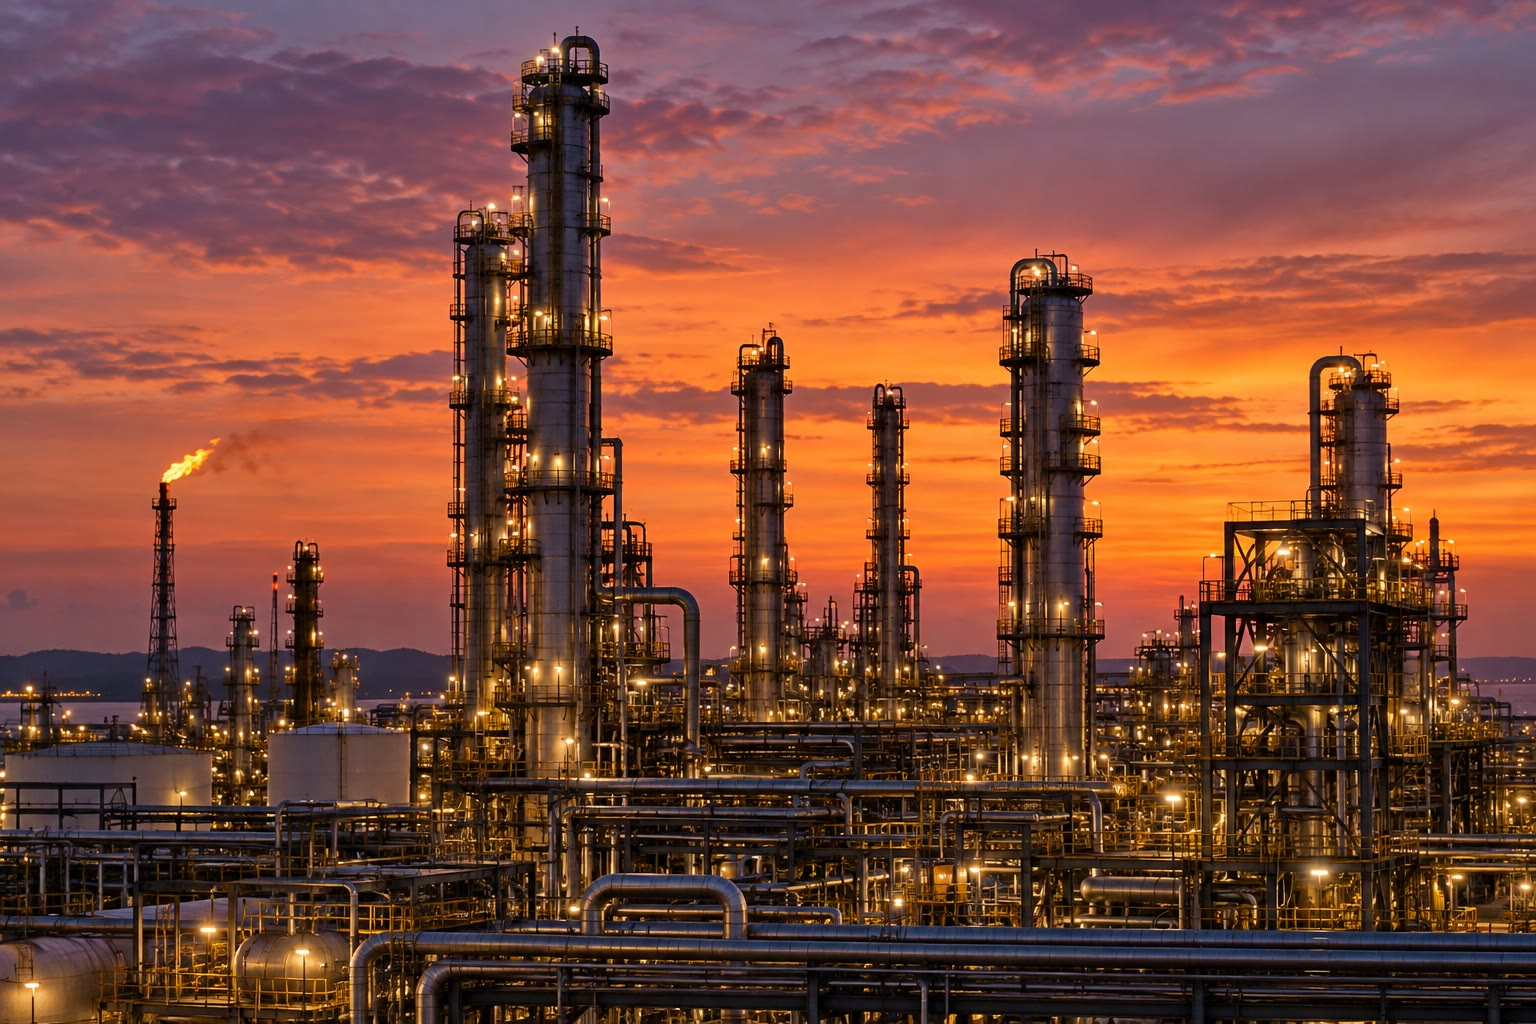
\includegraphics[width=0.52\linewidth]{images/book1/ai/g11-refinery-dusk.jpg}

{\small Columnas de \omterm{def:g10:chemical-species:distillation}{destilación} de una refinería al atardecer.}
\end{omfigure}

\begin{safety}{\ghs[0.66cm]{GHS02}\ghs[0.66cm]{GHS04}\ghs[0.66cm]{GHS07}\ghs[0.66cm]{GHS08}\ghs[0.66cm]{GHS09}}
% ledger: ghs:butane, ghs:pentane
El butano es un gas extremadamente inflamable, almacenado a presión. El
pentano es un líquido muy inflamable; sus vapores provocan somnolencia,
puede dañar los pulmones en caso de ingestión y es tóxico para los
organismos acuáticos. Ninguna llama cerca de los \omterm{def:g11:organic-skeletons:alkane}{alcanos} ligeros;
trabajar bajo una campana extractora.
\end{safety}

\section{Ejercicios}


\begin{exercise}[$\star$]\label{exo:g11:organic-skeletons:1}
Da las \omterm{def:g11:organic-skeletons:formulas}{fórmulas moleculares} de las \omterm{def:g7:atoms-and-molecules:molecule}{moléculas} dibujadas aquí, y di si son
\omterm{def:g11:organic-skeletons:isomer}{isómeros}:
\setchemfig{atom sep=1.6em}
\chemfig{-[:30]-[:-30]-[:30]-[:-30]-[:30]} \quad y \quad
\chemfig{-[:30](-[:90])-[:-30]-[:30]-[:-30]}.
\end{exercise}

\begin{exercise}[$\star$]\label{exo:g11:organic-skeletons:2}
Nombra: \ce{CH3-CH2-CH3}; \ce{CH3-CH2-CH2-CH2-CH2-CH3};
\chemfig{CH_3-CH(-[2]CH_3)-CH_2-CH_3}.
\end{exercise}

\begin{exercise}[$\star$]\label{exo:g11:organic-skeletons:3}
Escribe las \omterm{def:g11:organic-skeletons:formulas}{fórmulas semidesarrolladas} del propano y del
2-metilpropano, y la \omterm{def:g11:organic-skeletons:formulas}{fórmula estructural} del etano.
\end{exercise}

\begin{exercise}[$\star$]\label{exo:g11:organic-skeletons:4}
Cuenta los \omterm{def:g7:atoms-and-molecules:atom}{átomos} de carbono y de hidrógeno de cada \omterm{def:g7:atoms-and-molecules:molecule}{molécula}:
\setchemfig{atom sep=1.6em}
\chemfig{-[:30]-[:-30](-[:-90])-[:30]-[:-30]} \quad y \quad
\chemfig{*6(------)}.
\end{exercise}

\begin{exercise}[$\star$]\label{exo:g11:organic-skeletons:5}
Da la \omterm{def:g11:organic-skeletons:formulas}{fórmula molecular} del \omterm{def:g11:organic-skeletons:alkane}{alcano} de 8 \omterm{def:g7:atoms-and-molecules:atom}{átomos} de carbono, y el número
de \omterm{def:g7:atoms-and-molecules:atom}{átomos} de carbono del \omterm{def:g11:organic-skeletons:alkane}{alcano} de 20 \omterm{def:g7:atoms-and-molecules:atom}{átomos} de hidrógeno.
\end{exercise}

\begin{exercise}[$\star\star$]\label{exo:g11:organic-skeletons:6}
Dibuja las \omterm{def:g11:organic-skeletons:formulas}{fórmulas esqueléticas} del 3-metilhexano, el
2,2-dimetilbutano y el 3-etilpentano, y da sus \omterm{def:g11:organic-skeletons:formulas}{fórmulas moleculares}.
\end{exercise}

\begin{exercise}[$\star\star$]\label{exo:g11:organic-skeletons:7}
Dibuja y nombra los tres \omterm{def:g11:organic-skeletons:isomer}{isómeros} de \ce{C5H12}.
\end{exercise}

\begin{exercise}[$\star\star$]\label{exo:g11:organic-skeletons:8}
Estos nombres están mal. Dibuja cada \omterm{def:g7:atoms-and-molecules:molecule}{molécula} y da su nombre correcto:
2-etilbutano; 4-metilpentano; 1-metilbutano.
\end{exercise}

\begin{exercise}[$\star\star$]\label{exo:g11:organic-skeletons:9}
Con la figura de los \omterm{def:g11:organic-skeletons:isomer}{isómeros} de \ce{C5H12}, ordénalos por temperatura
de ebullición y explica el orden.
\end{exercise}

\begin{exercise}[$\star\star$]\label{exo:g11:organic-skeletons:10}
El ciclohexano es \ce{C6H12}, y el hexano, \ce{C6H14}. Explica los dos
\omterm{def:g7:atoms-and-molecules:atom}{átomos} de hidrógeno que faltan. ¿Son \omterm{def:g11:organic-skeletons:isomer}{isómeros} los dos compuestos? ¿Es el
ciclohexano un \omterm{def:g11:organic-skeletons:alkane}{alcano}?
\end{exercise}

\begin{exercise}[$\star\star$]\label{exo:g11:organic-skeletons:11}
Entre el propano, el butano, el 2-metilpropano y el ciclobutano
(\ce{C4H8}, un anillo de cuatro \omterm{def:g7:atoms-and-molecules:atom}{átomos} de carbono), ¿cuáles son \omterm{def:g11:organic-skeletons:isomer}{isómeros}
entre sí?
\end{exercise}

\begin{exercise}[$\star\star\star$]\label{exo:g11:organic-skeletons:12}
Dibuja y nombra los cinco \omterm{def:g11:organic-skeletons:isomer}{isómeros} de \ce{C6H14}.
\end{exercise}

\begin{exercise}[$\star\star\star$]\label{exo:g11:organic-skeletons:13}
Imagina un \omterm{def:g11:organic-skeletons:alkane}{alcano} lineal como un largo zigzag, y uno muy ramificado como
una bola. Con esta imagen, explica por qué la ramificación hace bajar la
temperatura de ebullición de los \omterm{def:g11:organic-skeletons:isomer}{isómeros}.
\end{exercise}

\begin{exercise}[$\star\star\star$]\label{exo:g11:organic-skeletons:14}
Nombra el \omterm{def:g11:organic-skeletons:alkane}{alcano}
\begin{center}
\chemfig{CH_3-CH(-[2]CH_3)-CH_2-C(-[2]CH_3)(-[6]CH_3)-CH_2-CH_3}
\end{center}
\end{exercise}

\begin{exercise}[$\star\star\star$]\label{exo:g11:organic-skeletons:15}
El compuesto de referencia para la gasolina, el ``isooctano'', es el
2,2,4-trimetilpentano. Dibuja su \omterm{def:g11:organic-skeletons:formulas}{fórmula esquelética}, comprueba que es
un \omterm{def:g11:organic-skeletons:isomer}{isómero} del octano y escribe su \omterm{def:g11:organic-skeletons:formulas}{fórmula semidesarrollada}.
\end{exercise}

\section{Problema: El gas de los mecheros}

\begin{problem}[{Problema de fin de semana --- ¿cuántos \omterm{def:g11:organic-skeletons:alkane}{alcanos}
distintos tienen la fórmula \ce{C7H16}?}]
\label{pb:g11:organic-skeletons:1}
% ledger: bp:C3H8, bp:C4H10, bp:isobutane
Un mechero contiene butano; un cartucho de camping de invierno contiene
una \omterm{def:g6:pure-substances-and-mixtures:mixture}{mezcla} más rica en propano o en 2-metilpropano. El butano hierve
hacia \qty{0}{\celsius}, el 2-metilpropano a \qty{-11.7}{\celsius} y el
propano a \qty{-42}{\celsius}.

\medskip
\noindent\textbf{Parte I --- Dos gases con una sola fórmula.}
\begin{enumerate}
  \item Da la \omterm{def:g11:organic-skeletons:formulas}{fórmula molecular} del butano, y comprueba que se ajusta a
        la fórmula general de los \omterm{def:g11:organic-skeletons:alkane}{alcanos}.
  \item Dibuja su \omterm{def:g11:organic-skeletons:formulas}{fórmula estructural}.
  \item Escribe sus \omterm{def:g11:organic-skeletons:formulas}{fórmulas semidesarrollada} y esquelética.
  \item Dibuja el 2-metilpropano de las mismas tres maneras. ¿Por qué
        tiene la misma \omterm{def:g11:organic-skeletons:formulas}{fórmula molecular}?
  \item ¿Son \omterm{def:g11:organic-skeletons:isomer}{isómeros} el butano y el 2-metilpropano? ¿De qué tipo?
\end{enumerate}

\medskip
\noindent\textbf{Parte II --- Con frío.}
\begin{enumerate}[resume]
  \item ¿Cuáles de los tres gases son gases a \qty{20}{\celsius} y a
        presión normal?
  \item Se usa un mechero abierto al \omterm{def:g4:air-a-mixture-of-gases:air}{aire} libre a \qty{-5}{\celsius}.
        ¿Por qué da una llama pobre?
  \item ¿Por qué los cartuchos de invierno son ricos en propano o en
        2-metilpropano?
  \item Explica por qué el 2-metilpropano hierve a menor temperatura que
        el butano.
  \item ¿Por qué el propano no tiene ningún \omterm{def:g11:organic-skeletons:isomer}{isómero}?
\end{enumerate}

\medskip
\noindent\textbf{Parte III --- Nombrar y contar.}
\begin{enumerate}[resume]
  \item Nombra \chemfig{CH_3-CH(-[2]CH_3)-CH_2-CH_3}.
  \item ¿Por qué el nombre ``3-metilbutano'' es incorrecto para la misma
        \omterm{def:g7:atoms-and-molecules:molecule}{molécula}?
  \item ¿Cuántos \omterm{def:g11:organic-skeletons:alkane}{alcanos} \omterm{def:g11:organic-skeletons:isomer}{isómeros} tienen las fórmulas \ce{C4H10},
        \ce{C5H12} y \ce{C6H14}?
\end{enumerate}

\medskip
\noindent\textbf{Parte IV --- Los \omterm{def:g11:organic-skeletons:isomer}{isómeros} de \ce{C7H16}.}
\begin{enumerate}[resume]
  \item Dibuja el \omterm{def:g11:organic-skeletons:isomer}{isómero} lineal y nómbralo.
  \item Dibuja y nombra los \omterm{def:g11:organic-skeletons:isomer}{isómeros} cuya cadena más larga tiene seis
        \omterm{def:g7:atoms-and-molecules:atom}{átomos} de carbono. ¿Por qué no existe el ``4-metilhexano''?
  \item Dibuja y nombra los \omterm{def:g11:organic-skeletons:isomer}{isómeros} cuya cadena más larga tiene cinco
        \omterm{def:g7:atoms-and-molecules:atom}{átomos} de carbono y dos grupos metilo.
  \item ¿Hay algún \omterm{def:g11:organic-skeletons:isomer}{isómero} con una cadena de cinco carbonos y un grupo
        etilo? ¿Por qué el grupo etilo solo puede estar en el carbono 3?
  \item Dibuja y nombra el \omterm{def:g11:organic-skeletons:isomer}{isómero} cuya cadena más larga tiene cuatro
        \omterm{def:g7:atoms-and-molecules:atom}{átomos} de carbono.
  \item Cuenta todos los \omterm{def:g11:organic-skeletons:isomer}{isómeros} encontrados.
  \item Da la respuesta final: ¿cuántos \omterm{def:g11:organic-skeletons:isomer}{isómeros constitucionales} tiene
        el heptano, incluido él mismo?
\end{enumerate}
\end{problem}
